\chapter{Distances} 
\label{chapter4-distances}

\section{Introduction}

In (\cite{memoli_comparing_2004}), four main categories of data analysis technique for high-dimensional data are compared, which are dimension reduction, clustering, regression analysis, and topological data analysis (TDA). Regarding choosing the appropriate distance in these methods, the paper (\cite{goos_surprising_2001}) examined the commonly used $L_p$ norm and showed that in high dimensional space, whether the notion of distance is qualitatively meaningful depends on the value of $p$.

In TDA, the relevant distance metric include the Gromov-Hausdorff distance, and on the space of persitence diagrams, the Bottleneck distance and the $p$-Wasserstein distance. In our application, we  followed closely the algorithm proposed in (\cite{kerber_geometry_2016}) to compute the $p$-Wasserstein distance between persistence diagrams. 

In this chapter, we will explain in detail the definitions and use cases of the above-mentioned distance metrics. The main references for this chapter are (\cite{chazal_introduction_2021}) and (\cite{phillips_notes}).

\begin{defn}[Metric Spaces]
Given a set $X$ and a function $d: X \times X \to \RR$, we say that the pair $\mathcal{M} = (X,d)$ is a \underline{metric space} on $X$ if and only if $d$ satisfies the following properties:

\begin{enumerate}
\item (Non-negativeness) For all $ x, y \in X, d (x, y) \geq 0.$
    \item (Identity) For all $ x, y \in X, d(x, y) = 0 \iff x = y.$
    \item (Symmetry) For all $x,y\in X, d(x, y) = d(y, x).$
    \item (Triangle Inequality) For all $x,y,z\in X, d(x, z) \leq d(x, y) + d(y, z)$.
\end{enumerate}

A point cloud is essentially a metric space $X$. Elements of $X$ are called points of the metric space. $d(x, y)$ refers to the distance between points $x$ and $y$. 
\end{defn}

\section{Distance between points in $\RR^d$}

\subsection{$L_p$ distance (Minkowski distance)}
\begin{defn}[$L_p$ distance]
Suppose $x, y \in \RR^d.$ Then the $L_p$ distance is defined as 
\begin{align}
    d_p(x,y) = \|x - y\|_p = \left(\sum_{i=1}^d(|a_i - b_i|^p)\right)^{1/p}.
\end{align}
\end{defn}

The following distance metrics are special instances of the $L_p$ distance. 

\begin{defn}[$L_2$ distance (Euclidean distance)]
The most common distance metric is the $L_2$ distance (or Euclidean distance). 
\begin{align}
      d_2(x,y) = \|x - y\|_2 = \left(\sum_{i=1}^d(|a_i - b_i|^2)\right)^{1/2}.
\end{align}
\end{defn}

\begin{defn}[$L_1$ distance (Manhattan distance)]
\begin{align}
      d_1(x,y) = \|x - y\|_1 = \sum_{i=1}^d(|a_i - b_i|).  
\end{align}
\end{defn}

Based on the paper (\cite{goos_surprising_2001}), in metric spaces with a high dimension, the $L_1$ distance and $L_p$ distance with fractional $p$ are more useful than the common $L_2$ distance. For this reason, in many computer vision tasks, the  $L_1$ distance is usually preferred. 

\begin{defn}[$L_\infty$ distance]
\begin{align}
      d_\infty(x,y) = \|x - y\|_\infty = \max_{i=1}^d |a_i - b_i|.
\end{align}
\end{defn}

The following figure compares the above instances of $L_p$ distance:
    \begin{figure}[H]
        \centering
            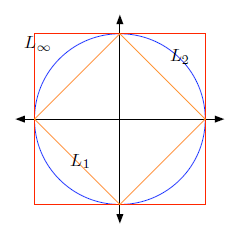
\includegraphics[width=0.5\textwidth]{figures/Lp-distances.png}
            \caption{Comparing the different $L_p$ distances. Adapted from (\cite{phillips_notes}).}
    \end{figure}

\subsection{Cosine distance}
The cosine distance measures the cosine of the angle between vectors $x,y\in \RR^d$
\begin{align}
    d_{cos}(x,y) = \frac{\xx \cdot \yy}{\|\xx\| \|\yy\|} = \frac{\sum_{i =1}^n x_i y_i}{\sqrt{\sum_{i =1}^n x_i^2} \sqrt{\sum_{i =1}^n y_i^2}}
\end{align}

\section{Distance between closed sets of points}

\begin{defn}[$\epsilon$-thickening]
Given a metric space $X$, the set of closed sets of $X$ supports a metric, the Hausdorff metric.

If $A$ is a set in $X$ and $\epsilon > 0$, we define the $\epsilon$-thickening of $A$ to be the set $A^{(\epsilon)}$ defined by

\begin{align}
    A^{(\epsilon)} =\bigcup_{x\in A} B_x(\epsilon),
\end{align}

where $B_x(\epsilon)$ is the open ball of radius $\epsilon$ centered at $x$. 
\end{defn}

\begin{defn}[Hausdorff distance]
    Suppose $A, B \subseteq X$ are closed sets, define their Hausdorff distance $d_H(A, B)$:
    
    \begin{align}
        d_H(A, B) =\inf\{\epsilon >0 \mid A\subseteq B^\epsilon \text{ and } B\subseteq A^\epsilon\}.
    \end{align}
\end{defn}

\begin{defn}[Gromov-Hausdorff distance]
The Gromov-Hausdorff distance extends the Hausdorff distance from subsets of the same metric space to subsets of distinct metric spaces.

Suppose $A, B$ are two closed metric spaces. Then the Gromov-Hausdorff distance is 
    \begin{align}
        d_{GH}(A,B) =\inf_{f,g}\{d_H(f_{A\to X}(A), g_{B\to X}(B))\},
    \end{align}
where $f_{A\to X}$ denotes an isometric embedding of $A$ into some metric space $X$ and $f_{B\to X}$ denotes an isometric embedding of $B$ into some metric space $X$. The infimum is taken over all possible such embeddings. 
\end{defn}

\section{Distance between persistence diagrams}
To make use of the topological features obtained from persistent homology, we need a distance metric to compare persistence diagrams. (\cite{kerber_geometry_2016})

\begin{defn}[Matching between persistent diagrams]
A matching between a pair of persistence diagrams $\dgm_1$ and $\dgm_2$ is a subset $M\subseteq \dgm_1 \times \dgm_2$ such that every point in $\dgm_1 $ and $\dgm_2$ appears exactly once in $M$. That is, for any $x\in \dgm_1$ and $y \in \dgm_2$, $(\{x\} \times \dgm_2) \cap M$ and $(\dgm_1 \times \{y\}) \cap M$ each contains a single pair. A matching is
perfect if every vertex is matched, that is, the matching is a bijection $\eta: \dgm_1 \to \dgm_2$. A perfect matching is illustrated in Figure \ref{fig:perfect-matching} below.
\end{defn}

The above definition has an equivalent formulation as an assignment problem:

\begin{defn}[Matching as assignment problem]
Given a weighted bipartite graph $G = (A \sqcup B,E,w)$, with $|A| = n = |B|$ and a weight function $w : E \to \RR_+$, a matching is a subset $M \subseteq E$ such that every vertex of $A$ and of $B$ is incident to at most one edge in $M$. 
\end{defn}
 
\begin{defn}[Bottleneck distance between persistent diagrams]
The \underline{Bottleneck distance} between a pair of persistence diagrams $\dgm_1$ and $\dgm_2$ is defined by
\begin{align}
    d_B(dgm_1, dgm_2) = \inf_M\{\max_{(x,y)\in M} \|x-y\|_\infty\},
\end{align}
where the infimum is taken over all possible matchings $M$.

If the matching is perfect, then the \underline{Bottleneck distance} can also be expressed as 
\begin{align}
    d_B(dgm_1, dgm2) = \inf_{\eta: \dgm_1 \to \dgm_2}\{\sup_{x\in\dgm_1} \|x-\eta(x)\|_\infty\},
\end{align}
\end{defn}

   \begin{figure}[H]
   \label{matching}
        \centering 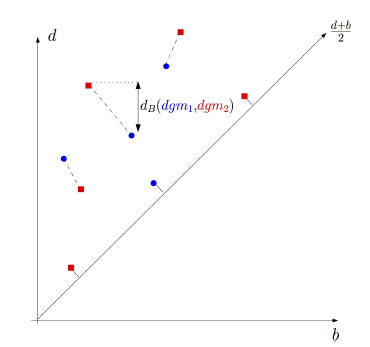
\includegraphics[width=0.5\textwidth]{figures/matching.png}
            \caption{A perfect matching and the Bottleneck distance between the blue and red persistent diagrams. Some points are matched to points on the diagonal. Adapted from (\cite{chazal_introduction_2021}).} \label{fig:perfect-matching}
    \end{figure}
 
\begin{defn}[$p$-Wasserstein distance between persistent diagrams]

Given $p\geq 1$, the $p$-Wasserstein distance between a pair of persistence diagrams $\dgm_1$ and $\dgm_2$ is defined by 
\begin{align}
    W_p(\dgm_1, \dgm_2) = \left(\inf_M \sum_{(x,y)\in M}\|x-y\|^p_\infty\right)^{1/p},
\end{align}
where the infimum is taken over all possible matchings $M$.
If the matching perfect, then the $p$-Wasserstein distance can also be expressed as 
\begin{align}
    W_p(\dgm_1, \dgm_2) = \left(\inf_{\eta: \dgm_1 \to \dgm_2} \sum_{x \in \dgm_1}\|x-\eta(x)\|^p_\infty\right)^{1/p},
\end{align}
As $p$ tends to infinity, the Wasserstein distance approaches
the bottleneck distance.

Note that in this report, when we use the term ``Wasserstein distance" interchangably with ``$p$-Wasserstein distance."
\end{defn}
\begin{defn}[$q$-tame persistence module]
A persistence module $\VV$ indexed by $T\subseteq \RR$ is $q$-tame if for any $r<s$ in $T$, the rank of the linear map $v^r_s: V_r\to V_s$ is finite.
\end{defn}

\begin{thm}[\cite{chazal_proximity_2009}]
If $\VV$ is a $q$-tame persistence module, then it has a well-defined persistence diagram. 
\end{thm}

\begin{thm}[Stability of persistence diagrams]
Let $\VV$ and $\WW$ 
be two $q$-tame persistence modules. If $\VV$ and $\WW$ are $\delta$-interleaved for some $\delta \geq 0$, then 
\begin{align}
    d_B(\dgm(\VV),\dgm(\WW)) \leq \delta,
\end{align}
\begin{align}
    W_p(\dgm(\VV),\dgm(\WW)) \leq \delta.
\end{align}
\end{thm}

Intuitively, the stability of persistence diagrams means that small perturbations in the persistence module will result in small perturbations in the Bottleneck distance and the $p$-Wasserstein distance between their respective persistence diagrams.

% \section{Comparing the different distances}
% This paper compares the four main categories of data analysis technique for high-dimensional data, each of which either defines or uses the distance metric differently:
% Dimension Reduction
% Clustering
% Regression analysis 
% Topological Data Analysis
